\chapter{Empurrando Juntos} \label{cap:empurrandojuntos}

A ideia da plataforma Empurrando Juntos surgiu no contexto do uso da Internet para
consolidação da democracia, o que \citeonline{penteadoencontro} resumiram como sendo o conceito de democracia digital.

Foi observado um viés nas discussões nas redes sociais há uma polarização das mensagens o que dificulta
a participação da minoria, ou seja, aqueles que pensam diferente dos demais. Dessa forma,
o objetivo da plataforma é dar voz para essa minoria e tornar as discussões mais efetivas para o propósito \cite{empurrandojuntos}. 


Essa participação 
acontece de duas formas: comentando uma conversa ou votando em um comentário de outro participante. Entende-se por voto
o ato de concordar com o comentário realizado (uma espécie de \textit{like}) ou discordar do comentário. Além disso, é permitido
que o usuário pule aquele comentário, ou seja, não atribua nenhum tipo de voto \cite{empurrandojuntos}. 

Com os votos realizados, é possível agrupar pessoas que responderam de maneira parecida, ou seja, concordaram e
discordaram dos mesmos comentários. Com os grupos formados, é possível ver a convergência e divergência de opiniões, 
prover ao usuário uma visão ampliada acerca do assunto e promover a interação entre os usuários com 
pensamentos divergentes. A Figura \ref{fig:resumo_ej} ilustra o funcionamento completo do sistema.

\begin{figure}[h!]
\centering
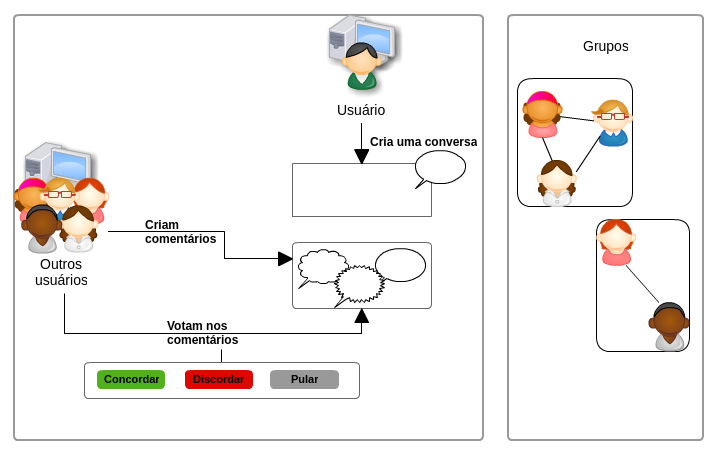
\includegraphics[scale=0.6]{figuras/resumo_ej.png}
\caption{Funcionamento do ``Empurrando Juntos''}
\label{fig:resumo_ej}
\end{figure}


